% Metódy inžinierskej práce

\documentclass[10pt,twoside,slovak,a4paper]{article}

\usepackage[slovak]{babel}
\usepackage[IL2]{fontenc}
\usepackage[utf8]{inputenc}
\usepackage{graphicx}
\usepackage{url}
\usepackage{hyperref} 

\usepackage{cite}

\title{Autopilot v robotických dronoch\thanks{Semestrálny projekt v predmete Metódy inžinierskej práce, ak. rok 2021/22, vedenie: Ing. Ján Lúčanský}}

\author{Alexej Putiška\\[2pt]
	{\small Slovenská technická univerzita v Bratislave}\\
	{\small Fakulta informatiky a informačných technológií}\\
	{\small \texttt{xputiska@stuba.sk}}
	}

\date{\small 14. december 2021}



\begin{document}

\maketitle

\begin{abstract}
Už v dnešnej dobe sa stretávame čím ďalej, tým viac s využitím dronov. Je to naozaj zariadenie budúcnosti. Kľúčom k prevádzke robotických dronov je softvér autopilota. Hľavným cieľom práce je zamerať sa na proces jeho fungovania. Popísať základný postup a prostriedky, ktoré sa využívajú pri ňom. Taktiež spomenúť momentálny a potencionálne budúci stav využiteľnosti autopilota dronov alebo ako sa pokúsiť zabezpečiť čo najbezpečnejšiu prevádzku. Okrem pozitívnych prínosov je zameraná aj na tie negatívne. Sú spomenúté hrozby, ktoré nám prinášajú, ale aj snaha o objektívne zodpovedanie na morálne otázky pri implementácii do bežného života a taktiež dopady na ľudskú spoločnosť.
\end{abstract}


\section{Úvod}
Dopyt po autonómnych zariadeniach v súčasnosti rastie. Osobitnou súčasťou autonómnych zariadení sú autonómne drony. Dron je možné vysvetliť ako bezpilotné lietadlo. Teda obrovskou výhodou je, že počas letu nie je ľudská bytosť jeho priamou súčasťou. Vďaka tomu sa spoločnosť snažila plne zautomatizovať prevádzku takéhoto zariadenia. Autonómne drony nie sú len vzdialená budúcnosť. Vďaka rýchlemu nárastu výkonných mikropočítačov je možné vytvárať veľmi pokročilé riešenia. \cite{smyczynski2017autonomous} Prevádzka a navigácia vo vonkajšom prostredí môže byť veľmi presná vďaka dostupnosti signálu GPS. Kooperatívny let v otvorenom priestore sa dá dobre vykonávať vďaka absencii prekážok, ktoré by mohli mať negatívny vplyv na komunikačné zariadenia. Lietanie v oblasti s väčším počtom prekážok, napr. vo vnútri budovy, je náročnejšie. Vyžaduje si veľmi presný pohyb v úzkych priestoroch so zakrytým alebo nedostupným signálom GPS. \cite{pestana2015vision} Vytvorenie autonómneho systému je veľmi náročné, pretože si vyžaduje integráciu viacerých prvkov, napr. plánovanie misie, navigáciu alebo mapovanie terénu. Existuje množstvo dostupných riešení pre tieto problémy samostatne, avšak integrácia týchto prvkov môže byť problematická. \cite{sanchez2017multi}


\section{Rozdelenie dronov na základe ich autonómnosti}
\begin{figure}[h]
	\label{fig:model1}
	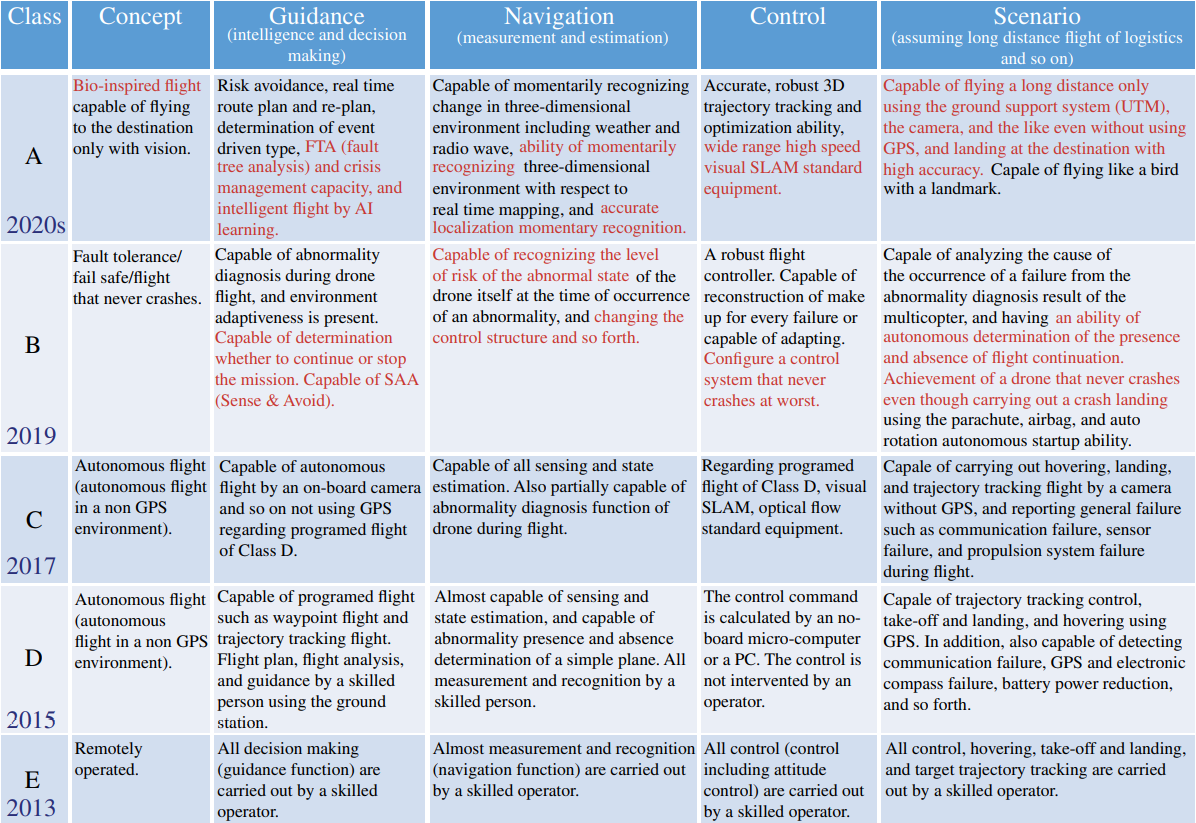
\includegraphics[width=\linewidth]{tabulka.png}
	\caption{Prehľad rozdelenia dronov na základe ich autonómnosti \cite{sanchez2017multi}}
\end{figure}
Na obrázku 1 je autonómia dronu, ktorá je takmer synonymom bezpečnosti, rozdelená do piatich stupňov od triedy A po triedu E, pričom pre každý z piatich stupňov je podrobne popísaná koncepcia, úroveň navádzania, úroveň navigácie, úroveň riadenia a scenár na základe predpokladu logistiky. \cite{sanchez2017multi} V ďalších podkapitolách sú stručne popisané charakteritiky každej zo spomínaných tried. 

\subsection{Trieda E}
Úroveň, ktorá je zavislá na obsluhe človeka pri rádiovo riadenej prevádzke dronu. \cite{nonami2020present}

\subsection{Trieda D}
Trieda, v ktorej je autonómny let možný ako naprogramovaný let, pri ktorom je všetko od vzletu po pristátie určené v pláne trajektórie, ktorý vopred vytvoril človek za predpokladu, že je možné prijímať rádiové vlny GPS. Všetko posudzuje kvalifikovaný človek. Je to trieda, v ktorej všetko spracúva palubná centrálna jednotka, automaticky oznamuje poruchu komunikácie, abnormality kompasu, zostávajúci stav batérie a podobne. \cite{nonami2020present}

\subsection{Trieda C}
Trieda C je určená pre drony schopné autonómneho letu aj v prostredí bez GPS. Využíva rôzne metódy, napríklad spracovanie obrazu pomocou kamery, lasera, lidaru, tachografu, zvukov a rádiových vĺn. Rôzne oznámenia o abnormalitách dronu a podobne sú podobné ako v triede D a prítomnosť a neprítomnosť pokračovania misie posudzuje človek. Najmodernejšie drony v roku 2017 patrili do triedy C. \cite{nonami2020present}

\subsection{Trieda B}
Drony sú definované ako stroje, ktoré nikdy nespadnú a v prípade abnormality autonómne rozvinú padák alebo podobne a vykonajú núdzové pristátie pred pádom. Na tento účel sa počas letu neustále aktivuje algoritmus na diagnostiku abnormalít a ak sa zdravotný stav lietajúceho robota líši od normálneho stavu, identifikuje sa príčina abnormality a autonómne sa posúdi, či sa bude v misii pokračovať alebo nie. \cite{nonami2020present}

\subsection{Trieda A}
Trieda A je ideálna forma lietajúceho robota, ktorú možno nazvať bioinšpirovaným letom, teda letom ako vták. Rádiové vlny GPS už nie sú potrebné. Vykonáva vysokorýchlostné spracovanie obrazu zo snímok zhotovených kamerou alebo podobným zariadením, ktoré je namontované na lietajúcom robotovi. Vykonáva tak odhad vlastnej polohy. Lietajúci robot je schopný sám rozpoznať, kde práve letí. Lietajúci robot má schopnosť dosiahnuť cieľ, ktorý je vzdialený aj 10 km alebo ďalej s orientačným bodom na zemi bez použitia rádiových vĺn GPS. Je to trieda, v ktorej lietajúci robot je schopný bezpečného letu tým, že vopred vníma abnormality lietajúceho robota pri vykonávaní analýzy porúch počas letu. V tejto fáze možno využiť aj efekt učenia sa umelej inteligencie, pričom čím viac lietajúci robot lieta, tým inteligentnejším sa autonómny let stáva. \cite{nonami2020present}


\section{Koncepcia ideálnej štruktúry autopilota}
Bezpilotné lietadlá sa používajú v čoraz väčšom počte civilných aplikácií, ako je napríklad kontrola a prieskum 
nebezpečných a zložitých prostredí, oblastí postihnutých katastrofou a podobne. Autonómne 
navádzanie, navigácia a riadenie sú potrebné na dosiahnutie týchto úloh bez priameho alebo 
nepretržitého ľudského riadenia.  \cite{nonami2010autonomous} 
	\begin{figure}[h]
	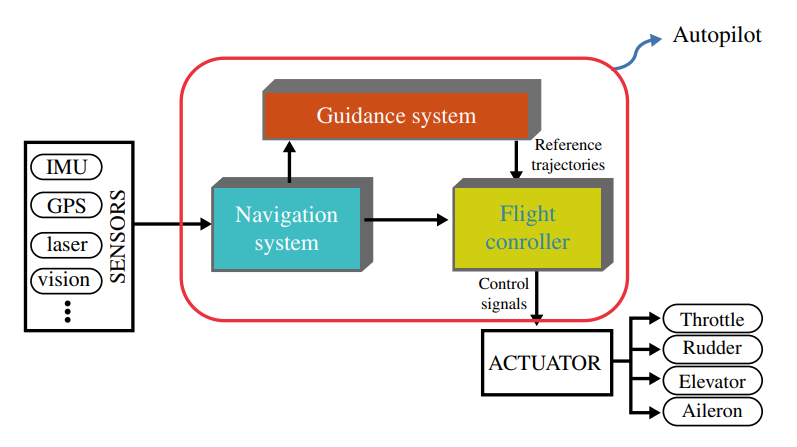
\includegraphics[width=\linewidth]{model.png}
	\caption{Ideálna štruktúra autopilota systému navádzania, navigácie a riadenia \cite{nonami2010autonomous}}
	\label{fig:model1}
	\end{figure}

Na obrázku 2 je znázornená jednoduchá bloková schéma systému navádzania, navigácie a riadenia.
Pozostáva z troch základných častí:
\begin{itemize}
\item Navigačný systém (Navigation system)
\item Systém navádzania (Guidance system)
\item Riadiaca slučka (Flight conroller)
\end{itemize} 

\subsection{Navigačný systém}
Navigačný systém je v širšom zmysle umenie určiť, kde sa nachádzate. V prípade autonómnych vozidiel, ako sú roboty a bezpilotné lietadlá, možno navigáciu definovať ako proces získavania informácií o vlastnom pohybe vozidla a tiež o okolitom prostredí. Tieto informácie môžu byť metrické (vzdialenosti) alebo typologické (orientačné body alebo akékoľvek iné podnety, ktoré sú užitočné na dosiahnutie úlohy a zaručenie bezpečnosti, napríklad použitie optického toku na vyhýbanie sa prekážkam). Navigačný systém zohráva v systéme lietadla kľúčovú úlohu. Štandardné navigačné algoritmy zvyčajne kombinujú informácie z mnohých zdrojov na odhad polohy, uhlových rýchlostí, výšky, rýchlosti a polohy vozidla vzhľadom na nejaký pevný referenčný bod alebo vzhľadom na nejaký cieľ. Pokročilé navigačné systémy zahŕňajú aj mapovanie, detekciu prekážok a lokalizáciu. Výstupy navigácie sa používajú pri navádzaní a riadení a ovplyvňujú výkonnosť letu a plnenie úloh. \cite{nonami2020present} \cite{nonami2010autonomous}

\subsection{Systém navádzania}
Navádzací systém možno definovať ako "vodič" drona, ktorý má splniť určitú úlohu. Prijíma vstupy z navigačného systému (kde sa nachádzam) a využíva informácie o zameraní (kam chcem ísť) na vyslanie signálov do systému riadenia letu, ktoré umožnia vozidlu dosiahnuť cieľ v rámci prevádzkových obmedzení vozidla. Navádzací systém má teda za úlohu plánovať dráhu letu a generovať požadované stavové vektory (poloha, rýchlosť, smer a výška), ktoré musí vozidlo sledovať. Medzi základné ťažkosti patrí čiastočne známe a meniace sa prostredie, cudzie faktory, ako sú hrozby, a výpočtová zložitosť, pretože problém plánovania trajektórie sa vo všeobecnosti rieši pomocou matematických optimalizačných metód, ktoré sú výpočtovo príliš náročné. \cite{nonami2020present} \cite{nonami2010autonomous}

\subsection{Riadiaca slučka} 
Riadiaca slučka prijíma navádzacie príkazy a využíva navigačné údaje na generovanie aktuálnych signálov pre pohyb drona, ako aj na stabilizáciu polohy vozidla. Túto časť je teda možné predstaviť ako miesto, kde sa zlepujú získané informácie a prenášajú sa až do samotného pohonu, ktorý uvedie dron do požadovaného pohybu. \cite{nonami2020present} 

\section{Reakcia na témy z prednášok}
\paragraph{Technológia a ľudia.} Vysnívaný stupeň autonómnosti dronov spôsobí to, že ich bude môcť ovládať naozaj každý. S takým robotom sa budeme stretávať denne. Plne zautomatizovaný autonómny dron nahradí niektoré pracovné pozície, ako napríklad profesia kuriéra bude vo veľkej miere odlišná. Trh práce sa zmení, a preto sa dá povedať, že zavedenie dronov do bežného života môže byť prelomový okamžik v spôsobe života ľudí. 
\paragraph{Historické súvislosti.} Navádzacie a navigačné systémy boli pôvodne vyvinuté pre rakety. Tieto systémy získali širšie využitie s príchodom kozmických lodí, riadených striel a bezpilotných lietadiel. \cite{nonami2018all} Ako pri množstve vynálezov aj autonómne drony mali zo začiatku len malý okruh využiteľnosti. Avšak sa postupom času začínali využívať viac, ako napríklad aj na zábavu, a v blízkej budúcnosti budú pravedobne súčasťou každodenného života.  
\paragraph{Udržateľnosť a etika.} Už v tomto období je zrejmé, že pokrok v oblasti autonómnych dronov sa nezastaví. Pri premýšľaní nad tým, sa naskytne aj otázka, či to pôjde správnym smerom. Princípy autonómnosti majú svoj vznik vo vojenskom priemysle, a preto jasné, že v tejto oblasti ich vývoj bude aj pokračovať. A teda, využije sa taký skvelý prostriedok na nemorálne účely? S určitosťou je možné povedať áno. Dokonca sa už aj k takýmto účelom využíva, aj keď sa s tým väčšina z nás nestretla. Autonómne drony môžu buď pozitívne uľahčovať život ľudí, alebo viesť k úplnej strate súkromia a byť aktívnou súčasťou vojenských konfliktov. Je len na spoločnosti ako sa k tomu postaví.

\section{Záver}
Od dronov sa vyžaduje spoľahlivosť, odolnosť a bezpečnosť, ktoré im umožnia opakovať denný let v trvaní približne 8 hodín po dobu približne 5 rokov. Netreba spomínať samozrejmý postup každodennej pravidelnej kontroly a výmeny komponentov. Lietajúci robot blízkej budúcnosti je pokročilý intelektuálny lietajúci stroj, ale aj po splnení takých predpokladov stále zostáva strojom. Takže lietajúci robot, ktorý lieta veľmi nízko, kde sa počasie zvykne drasticky meniť, musí mať funkciu schopnú reagovať na abnormálne udalosti počas letu. Autonómny dron novej generácie musí byť "dronom, ktorý nikdy nehavaruje", ale pred haváriou vykoná núdzové pristátie na bezpečnom mieste, ktoré on sám vyhľadá. V tomto zmysle takýto lietajúci robot ešte nebol uvedený na trh. Autonómne drony sa však vyvíja tak rýchlo, že v najbližších rokoch budú mať autonómiu triedy A. \cite{nonami2020present}



\bibliography{literatura}
\bibliographystyle{plain} 
\end{document}
